\documentclass[12pt, titlepage]{article}

\usepackage{float}
\usepackage{booktabs}
\usepackage{tabularx}
\usepackage{hyperref}
\usepackage{graphicx}
\usepackage{titling}
\usepackage[utf8]{inputenc}
\usepackage{graphicx}
\usepackage{gensymb}
\usepackage{siunitx}
\usepackage{textcomp}
\usepackage{longtable}
\graphicspath{{./images/}}
\usepackage{array}
\graphicspath{ {figures/} }

\hypersetup{
    colorlinks,
    citecolor=black,
    filecolor=black,
    linkcolor=blue,
    urlcolor=blue
}
\usepackage[round]{natbib}
\begin{document}

\title{
    MobiCharged\\Module Guide 
    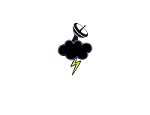
\includegraphics[width=9cm]{images/mobicharged.png} 
}
\author{Team Super Charged (No.33)
		\\ Nashit Mohammad - mohamn31
		\\ Eric Nguyen - nguyee13
		\\ Samuel De Haan - dehaas1
		\\ Eamon Earl - earle2
		\\ Mustafa Choueib - choueibm
}
    

\date{April 4th, 2023}


\maketitle

\pagenumbering{roman}
\tableofcontents
\listoffigures
\listoftables

\vspace{20pt}
\begin{center}
\begin{table}[H]
\caption{\bf Revision History}
    \begin{tabular}{p{2cm}p{3cm}p{2cm}p{6cm}}
    \hline
    \bf Author & \bf Date & \bf Version & \bf Description\\
    \hline
    All & April, 2023 & Rev 1 & Created final draft of Document \\
    \hline
    \end{tabular}
\end{table}
\end{center}

\newpage

\pagenumbering{arabic}

\section{System Overview}

\subsection{Naming Conventions and Terminology}

\begin{table}[htp]
\caption{\bf Naming Conventions and Terminology}
\begin{tabular}{ |p{6cm}|p{8cm}|  } 
 \hline
\bf Word/Acronym & \bf Definition/Context\\
 \hline
 Functional Requirement & Requirements that describe what the product is supposed to do\\
 \hline
Non-functional Requirement & Requirements that describe qualities that product will have\\
 \hline
General Contractor & Third party companies that acquire services by Mobilite-Power\\
 \hline
Data Smoothing & The process of using old data as well as "future" data in order to predict designs\\
 \hline
ML & "Machine Learning" algorithm\\
\hline
AC & Ancticipated Change\\
\hline 
R & Requirement\\
\hline 
UC & Unlikely Change\\
\hline 
A & Assumption\\
\hline 
DS & Download Speed\\
\hline
US & Upload Speed\\
\hline
I/O & Input/Output\\
\hline
\end{tabular}
\end{table}

\subsection{Relevant Facts and Assumptions}
\begin{itemize}
    \item There is an assumption that the developers will eventually have access to enough processing power to conduct large quantities of simulations.

\end{itemize}

\subsection{Introduction}

Engineers are tasked with design in construction to exceed expecations without hindering safety. Safety is a topic that is never missed within the industry and is continuously being highlighted amongst designs; especially as Engineers are reminded of their moral obligations to society by their awarded rings upon graduation. 
\par
As a current process, the construction industry places sensors within concrete spaces to continuously test and/or monitor the integrity of buildings during as well as after construction. Ultimately however, these sensors run out of battery and are required to be re-charged.
\par
The industry still faces challenges when attempting to charge these sensors with the method of remote charging as the current products that satisfy remote charging abilities are yet to be optimized. There are a significant number of buildings being built in the Greater-Toronto-Area, which is emphasized considering that 70\% of cranes within Canada are in just the GTA alone. To place innovation in the sub-field of safety within the industry, it is indeed a requirement to modernize the ability of producing efficient remote charging systems and to have the design process optimized to provide the most effective results.
\par
The system-solution for this will be the development of MobiCharged. 



\section{Module Hierarchy}
\subsection{Software System Module Hierarchy}
For the machine learning algorithm to be effective, it is efficient for it to be modularized. Below is a list and diagram of the software system module hierarchy, where further information upon these modules are outlined in the Module Decomposition section.

\subsection{Modules}
\begin{itemize}
  \item Input Module
  \item Initializer Module
  \item Machine Learner Blackboard Indirection Layer
  \item Database Access Module 1
  \item Database Access Module 2
  \item User Interface Module
  \item Controller / Server Module
  \item “Client” Module
\end{itemize}

\begin{figure}[htp]
  \centering
  \includegraphics[width=7cm]{images/Figure1.png}
  \caption[Software Architecture Modules]{Software Architecture Modularized }
  \label{fig:figure1}
\end{figure}

\subsection{Hardware Module Hierarchy}
Although the physical simulation component of this project is not connected to the software portion directly, the hardware system can still be modularized to exhibit the workings of the system.
\par 
Below is a high-level module hierarchy of the hardware system where further information on each module will be described in the Module Decomposition section. Please note that the “modules” here can be more thought of to be component sections.
\par

\begin{itemize}
  \item Electronic circuitry (includes MOSFET drivers, capacitors \& transducers i.e. electrosonic emitters)
  \item Microcontroller Module
  \item Power Supply Module (includes connectors \& ports)
  \item Shaped 3D Printed Case
\end{itemize}

For further illustrations of the components of the hardware system, below are diagrams depicting the connection between components.
\par 

\begin{figure}[htp]
  \centering
  \includegraphics[width=7cm]{images/Figure2.png}
  \caption[PCB and Power]{PCB Board Component with FPGA \& Power Requirements}
  \label{fig:figure2}
\end{figure}

As shown in figure 8 above, output pins of the Arduino Nano will be used to control the driver. The driver board will be powered by an external power supply and will be used to boost the signals from the Arduino. The driver has two output channel. Each will control an individual array.
\par 
The arrays will be connected to the driver as shown in figure 8. Each concentric ring of transducers will be wired in parallel. One of the channels will be held constant, however the others phase will be able to be changed by the controlling software in order to impliment verticle movement.
\par
The constructed shape of the 3D printed casing will work as psuedo-phase shifters. The offset of the verticle placement of the transducers in the case work to create the interference required for acoustic levitation. 

\section{Module Decomposition}
\subsection{Software Module Decomposition}
\begin{longtable}{|p{2cm}|p{3cm}|p{3cm}|p{3cm}}
  \caption{\bf Software Modules}\\
    \hline
    \bf Module & \bf Service & \bf Secret & \bf Estimated Completion\\
    \hline
    Initializer Module & Initializes main loop, and databases.  Allocates space for data processing, verifies that the MATLAB simulation compiles. Bounces errors if memory cannot be allocated or if MATLAB does not compile.  & The number of inputs/outputs that will determine how much memory is allocated, and the errors that can be returned. & End of January 2023. This module is finished for the most part. It may require slight edits when implementing with the other modules.\\
    \hline 
    Controller/ Server Module & Handles communication between the “Server” and “Client”. Passes inputs based on provided boundaries to Client module and returns optimal outputs. & The simulation inputs passed to client and the optimal outputs received by the client. & End of January 2023. This module is finished for the most part. It may require slight edits when implementing with the other modules.\\
    \hline 
    Client Module & Client module receives inputs and passes through MATLAB simulation and returns optimal outputs. & The MATLAB simulation format, simulation inputs and outputs. & End of January 2023. This module is finished for the most part. It may require slight edits when implementing with the other modules.\\
    \hline 
    Machine Learner Blackboard Indirection Layer & Reads batches of data from Database Access Module 1. Once certain data thresholds have been reached, this module passes batched data to specific model training streams. During downtimes where the amount of new data is received, this module will run validation test suites to monitor progress of models. Allows user requests for input into predictive models. This module will ultimately filter out the best performing models. & The data that is read from Database Access Module 1, format of validation tests, user requests, and trained models. & Feb-March. A large amount of simulation data still needs to be produced in order to train and test models.\\
    \hline 
    Database Access Module 1 & Stores the generated inputs and corresponding optimal output. Establishes basic reading and writing concurrency control. & The simulation inputs and optimal outputs that are stored in this database. & End of January 2023. This module is completed for the most part. However, the formatting of the database may require editing when simulation data is produced.\\
    \hline 
    Database Access Module 2 & Stores the generated hyperparameters and performance of each model stream in the Machine Learner Blackboard Indirection Layer. & The hyperparameters and model performances stored in this database. & Feb-March. A large amount of simulation data still needs to be produced in order to train and test models.\\
    \hline 
    User Interface Module & Controls the communication of the user prediction requests to the Machine Learner Blackboard Indirection Layer. It also displays the model performances after each validation test trial. & The results of the validation tests on the models, and the user requests. & Feb-March. This module requires the Machine Learner Blackboard Indirection Layer to be completed first. \\
    \hline 
\end{longtable}
\subsection{Hardware System Module / Component Timelines}
The following table will outline the dates of completion for the hardware modules.
\begin{table}[htp]
  \caption{\bf Hardware System Timeline}
      \begin{tabular}{|p{4cm}|p{4cm}|}
           \hline
           \bf Module & \bf Estimated Completion\\
           \hline
           3D Printed casing & Jan 20th, 2023\\
           \hline
           Elctronic circuitry & Jan 28th, 2023\\
           \hline
           Microcontroller Module & Feb 3rd, 2023\\
           \hline 
           Power Supply Module & Jan 20th, 2023\\
           \hline 
      \end{tabular}
  \end{table}

\section{Traceablility Matrix}
The following is the traceablility matrix for the software system.
\begin{longtable}{|p{4cm}|p{4cm}|}
  \caption{\bf Traceablility Matrix}\\
           \hline
           \bf Module & \bf Requirements\\
           \hline
           Initializer Module & ACR1\\
           \hline
           Machine Learner Blackboard Indirection Layer & SR1, SR2, SR3, SR5, SR6, PAR1, RAR1\\
           \hline 
           Database Access Module 1 & IR1, RAR1, RFTR1, PRV1\\
           \hline 
           Database Access Module 2 & IR1, RAR1, RFTR1, PRV1\\
           \hline 
           Controller/Server Module & SR5\\
           \hline 
           Client Module & SR4, ACR1, IR1, ADAR1\\
           \hline 
           User Interface Module & APR1, ACR1, EUR1, EUR2, LR1, SLR1, RAR1, ADAR1\\
           \hline 
  \end{longtable}

\section{Anticipated and Unlikely Changes}

\begin{longtable}{|p{4cm}|p{4cm}|}
  \caption{\bf Anticipated Changes}\\
           \hline
           \bf Module & \bf Anticipated Changes\\
           \hline
           Initializer Module & The number of inputs/outputs and their bounds will change once the MATLAB simulation format is finalized.\\
           \hline
           Machine Learner Blackboard Indirection Layer & The range of model architectures will change as we gain insight on what types of models perform the best with the simulation data. The batch size of the data being read and the data thresholds will also change.\\
           \hline 
           Database Access Module 1 & The formatting of this database will change if the MATLAB simulation format changes. For example, the simulation may be changed to add or remove features in the data.\\
           \hline 
           Database Access Module 2 & The formatting of this database may change as new model architectures are tested.\\
           \hline 
           Controller/Server Module & The formatting of the inputs and outputs sent and received from the client will change depending on the MATLAB simulation file.\\
           \hline 
           Client Module & The formatting of the inputs and outputs sent and received from the client will change depending on the MATLAB simulation file.\\
           \hline 
  \end{longtable}

\begin{longtable}{|p{4cm}|p{4cm}|}
  \caption{\bf Unlikely Changes}\\
           \hline
           \bf Module & \bf Unlikely Changes\\
           \hline
           Initializer Module & Handling memory storage and error calls as this is necessary and currently most efficient to be instilled within this module\\
           \hline
           Machine Learner Blackboard Indirection Layer & During downtimes where the amount of new data is received, this module will run validation test suites to monitor progress of models. This is unlikely to change in order to maximize efficiency as well as accuracy of results.\\
           \hline 
  \end{longtable}

\section{Use Hierarchy between Modules}
The figure below displays the use cases between the modules (eg: Optimal I/O module depends on the Initializer module to work).
\begin{figure}[htp]
  \centering
  \includegraphics[width=7cm]{images/Figure1.png}
  \caption[Uses Hierarchy]{Uses Hierarchy for Software System}
  \label{fig:figure3}
\end{figure}


\section*{References}
SRS, \url{https://github.com/SamueldeHaan/MobiCharged/blob/main/docs/SRS/SRS.pdfs}
Design Document, \url{https://github.com/SamueldeHaan/MobiCharged/blob/main/docs/Design/DD_REV_0.pdfs}
MIS, \url{https://github.com/SamueldeHaan/MobiCharged/blob/main/docs/Design/MIS/MIS.pdfs}

\bibliographystyle{plainnat}

\bibliography{Design Document}

\newpage

\newpage{}
\section*{Appendix --- Reflection}

The information in this section will be used to evaluate the team members on the graduate attribute of Problem Analysis and Design. Please answer the following questions: 
\par 
\begin{enumerate}
  \item What are the limitations of your solution? Put another way, given unlimited resources, what could you do to make the project better? (LO ProbSolutions) 
  \item Give a brief overview of other design solutions you considered. What are the benefits and tradeoffs of those other designs compared with the chosen design? From all the potential options, why did you select documented design? (LO Explores)
\end{enumerate}

\begin{enumerate}  
  \item The limitations of our solution is primarily cost \& time. \par The problem of making the process of obtaining data values for the purpose of creating remote charging devices specific to certain applications easier is proposed to be solved through the methods of machine learning algorithms. That is, the process would become significantly easier if a machine learning algorithm could output the data values necessary at a much faster speed (and subsequently lower computational costs) without the use of simulations. \par The proposed solution has limitations in verifications. Through the original method of using simulations, the consequence is that it is extremely timely to output. However, the benefit of it is exhibited with verification of values. Through the machine learning algorithms, although the speed of the values being outputted increases significantly, the idea of verification becomes lost; particularly in the case where the algorithm goes past the limits of inputs provided. \par Given unlimited resources, the solution could become better if more time was present such that modules were created that verify the values and provide higher certainty in the values outputted. 
  Moreover, more servers would be purchased so that it may feed the machine learning algorithm without the use of users inputting data manually (referring to the client modules). \par 
  In regards to the hardware system, the proposed solution would become better with appropriate equipment to create a real prototype as opposed to a simulative one. The prototype would be better for display as well as feeding limits to the software by purchasing equipment such as antenna arrays, phase arrays, electromagnetic wave resistant encapsulations, etc. Moreover, with unlimited resources, the hardware system would be given an embedded system such that it may direct “charging” signals remotely to desired devices.
  \item An alternative solution for the design of this project was manually obtaining values based on certain inputs (and subsequently certain applications) over a wide range such that we may feed it into the machine learning algorithm. Although the benefit of this method is that the values are verified, it was better thought of to use a single server or two in order to run these simulations continuously in the backend automatically. This way, it is more efficient obtaining the values in the long term. In addition, this would be more effective for our client Mobilite Power as they can use the architecture of our software system and feed their large data set into it. This way, the machine learning algorithm will output more accurate results over a wider range of data. \par 
  Regarding the hardware system, an alternative solution was to create a small charging device using a pre-purchased antenna array. This would be done without the phase arrays but be implemented with a larger structure around the system to solve our stretch goals (which include being resistant to weather conditions). The benefit in this is that we can display different antenna array shapes \& sizing while illustrating the change in results; which we predicted to be power distributed as well as accuracy of electromagnetic waves sent. The problem with this solution is the limitation of resources. The group proceeded with creating a simulation of a remote charging device using a phased array system with the fear that the original solution mentioned would not be completed in a timely manner due to the expertise required. The original solution would dive into the area of PHD level projects and would be a risk in completion.   

\end{enumerate}


\end{document}

